\begin{frame}{Introduction}{Motivation}
    \begin{itemize}
        \setbeamercovered{transparent}
        %\onslide<1->{\item The term \textit{open data} nowadays is popularized and becomes trending in many cities or nations around the world.}
        \onslide<1->{\item Building a smart city or electronic government trend.
              % requires a huge amount of data sets.
              }
              % Sharing data between a federal or citizens is an efficient method that can save time and effort for data preparation
              \onslide<2->{\item The security aspects of \textit{open data} -- CIA triangle.}
    \end{itemize}
    \uncover<3->{
        \begin{figure}
            \centering
            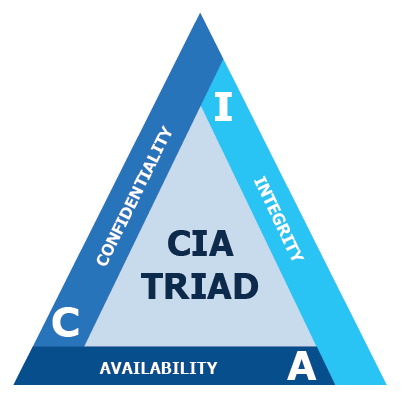
\includegraphics[width=.3\textwidth,height=.3\textwidth]{img/CIA-Triangle-02.png}
            % \caption{Open data}
            %   \label{fig:arOv}
        \end{figure}
    }
    \begin{itemize}
        \setbeamercovered{transparent}
        \onslide<3->{
        %   \item Attacking on websites or databases have been going on and inflict tremendous damage because of centralize system disadvantage.\\
        \onslide<4->{\item Centralize system disadvantage \\
              \uncover<5->{$=>$ Invalid data sets led people to make bad decisions.}
              }
              }
    \end{itemize}
\end{frame}
\begin{frame}{Introduction}{Motivation}
    Here are a few famous attacks since 2008\footnote{https://www.itsecurityguru.org/2016/11/29/2017-year-data-integrity-breach/}:
    \begin{itemize}
        \item 2008 - Hackers infiltrate the Brazilian governments systems and inflate the logging quotas to disrupt logging industry.
        \item 2010 - Hackers use the Stuxnet Worm to make minor changes in Iran’s nuclear power program in an attempt to destroy it.
        \item 2015 - Anonymous begin releasing financial reports exposing firms in the US and China trying to cheat the stock market.
              % In one case, damaging the brand reputation of REXLot Holdings, a games developer, which had inflated its revenues
        \item 2015 - JP Morgan Chase was breached with subsequent attempts at market manipulation.
        \item 2016 - Both the World Anti-Doping Agency and Democratic National Committee are breached with hackers manipulating their data to embarrass the organisations.
    \end{itemize}
\end{frame}

% \begin{frame}{Introduction}{Solution}
%     \setbeamercovered{transparent}
%     \begin{itemize}

%         % \item<2-> Blockchain and open data: a match made in heaven?
%         \onslide<1->{\item \textbf{Our idea}: Blockchain + IPFS +  Open data.}
%     \end{itemize}
%     \begin{figure}
%         \centering
%         \includegraphics<2->[width=.6\textwidth,height=.25\textwidth]{img/intro.png}
%         % \caption{Open data}
%         % \label{fig:arOv}
%     \end{figure}
% \end{frame}
